\documentclass[10pt]{article}
\usepackage{../../local}


\newcommand{\classcode}{Physics 137B}
\newcommand{\classname}{Quantum Mechanics II}
\renewcommand{\maketitle}{%
\hrule height4pt
\large{Eric Du \hfill \classcode}
\newline
\large{HW 11} \Large{\hfill \classname \hfill} \large{\today}
\hrule height4pt \vskip .7em
\normalsize
}
\linespread{1.1}
\begin{document}
	\maketitle
	\section*{Collaborators}
	I worked with \textbf{Andrew Binder} to complete this assignment. 

	\section{Problem 1}
	Derive the Optical theorem: $\sigma = \frac{4\pi}{k}\Im(f(0))$


	\begin{solution}
		We know the existence of the following form for the optical theorem: 
		\[
			\sigma = \frac{4\pi}{k^2}\sum_{l = 0}^\infty (2l + 1)\sin^2 \delta_l
		\] 
		To prove the optical theorem, we plug in $\theta = 0$ into the normal scattering amplitude: 
		\[
			f(\theta) = \frac{1}{k}\sum_{l=0}^\infty (2l + 1)P_l(\cos \theta) e^{i \delta_l} \sin \delta_l 
		\] 
		Notice that this will cause $\cos \theta = 1$, and since $P_l(1) = 1$ for all Legendre polynomials, 
		then this will kill off all the Legendre polynomial terms. Then, taking the imaginary part, we 
		take the $\sin \delta_l$ component of $e^{i \delta_l}$. Therefore: 
		\[
			\Im(f(0)) = \frac{1}{k}\sum_{l = 0}^\infty (2l + 1)(\sin \delta_l) \sin \delta_l = \frac{1}{k}
			\sum_{l = 0}^\infty (2l + 1) \sin^2 \delta_l
		\] 
		Then, multiplying this by $\frac{4\pi}{k}$ in order to get the original expression for $\sigma$, we get:
		\[
			\sigma = \frac{4\pi}{k^2}\sum_{l = 0}^\infty (2l+1) \sin^2 \delta_l
		\] 
		As desired.
	\end{solution}
	\pagebreak

	\section*{Problem 2}
	\begin{enumerate}[label=\alph*)]
		\item At a center-of-mass energy of 5 MeV, the phase shifts describing the elastic scattering of a
			neutron by a certain nucleus have the following values:
			\[
			\delta_0 = 32.5^\circ , \ \ \delta_1 = 8.6^\circ \ \ \delta_2 = 0.4^\circ
			\] 
			Assuming all other phase shifts to be negligible, plot $\dv{\sigma}{\Omega}$ as a function of 
			scattering angle. what is the total cross section $\sigma$? For simplicity take the reduced mass of 
			the system to be that of the neutron. 

			\begin{solution}
				We use the expansion of $f(\theta)$ from the partial wave analysis:
				\[
					f(\theta) = \sum_{l = 1}^\infty (2l+1)P_l(\cos \theta) e^{i \delta_l} \sin \delta_l
				\] 
				Then, since the problem tells us that the contribution from $l > 2$ is negligible, we can 
				just take the sum from $l = 0, 1, 2$ terms. Since there are only three terms here, I just 
				plugged each $\delta_i$ into python, obtained $f(\theta)$ in this way, then used the relation:
				\[
					\dv{\sigma}{\Omega} = |f(\theta)|^2
				\] 
				to calculate the differential cross section. Doing so, we get the following plot using the 
				$\delta_i$ given in the problem:
				\begin{center}
					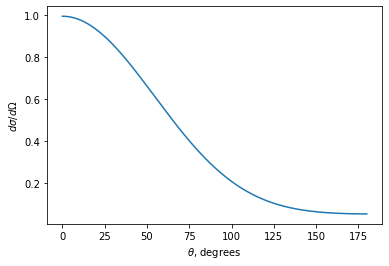
\includegraphics[scale=0.8]{q2a.png}
				\end{center}
				To calculate the total cross section, we have to take this integral over all $\theta$. I
				did this part numerically (since I plotted in python), so I'll show the cross section there.
			\end{solution}
		\item the same if the algebraic sign of all three phase shifts is reversed. 

			\begin{solution}
				All we have to do here is alter the initial $\theta$ given. This plot looks like:
				\begin{center}
					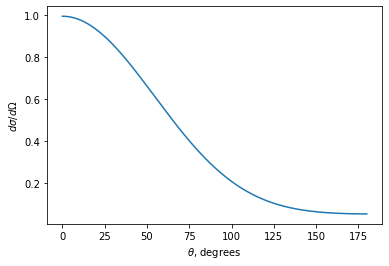
\includegraphics[scale=0.8]{q2b.png}
				\end{center}
				Notice that this plot looks the same as the one from part (a).
			\end{solution}
		\item The same if the sign of only $\delta_0$ is reversed.

			\begin{solution}
				Again, we do the same thing as part (a) but plug in different $\delta_i$ values:
				\begin{center}
					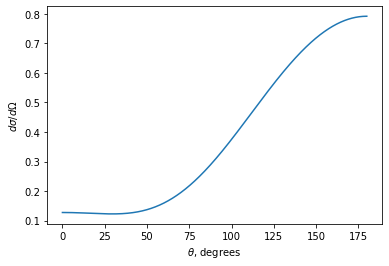
\includegraphics[scale=0.8]{q2c.png}
				\end{center}
			\end{solution}
		\item Using the results of part (a), calculate the \textit{total} number of neutrons scattered per
			second out of a beam of $10^{10}$ neutrons per $\text{cm}^2$ per sec, of cross sectional area 
			$2 \text{ cm}^2$, incident upon a foil containing $10^{21}$ nuclei per $\text{cm}^2$ How many
			neutrons per second would be scattered into a counter at $90^\circ$ to the
			incident beam and subtending a solid angle of $2 \times 10^{-5}$ ster-radians?

			\begin{solution}
				Here, we use the relation that $N_{sc} = N_{inc}n_{tar} \sigma$, so all we have to do is 
				compute $\sigma$. Computing the numerical integral, we get the cross section $\sigma = 8.34
				\times 10^{-24}$. Therefore, this means that the total number of neutrons scattered: 
				\[
					N_{sc} = (2 \times 10^{10})(10^{21}) (3.253 \times 10^{-25}) = 650600
				\] 
				As for $\theta = \frac{\pi}{2}$, we get that the scattering cross section over an angle of 
				$2 \times 10^{-5}$ ster-radians is $\sigma = 2.263 \times 10^{-31} \text{cm}^2$, so therefore:
				\[
					N_{sc} = (2 \times 10^{10})(10^{21})(2.263 \times 10^{-31}) = 4.526
				\] 
				So we can see that about one sixth of the incident particles scatter and hit the detector
				at an angle of $90^\circ$.
			\end{solution}
	\end{enumerate}
	\pagebreak

	\section*{Problem 3}
	Analysis of the scattering of particles of mass $m$ and energy $E$ from a fixed scattering center with 
	characteristic length $a$ finds the phase shifts
	\[
		\delta_l = \sin^{-1} \left[ \frac{(iak)^l}{\sqrt{(2l + 1)l!} }\right]
	\] 
	\begin{enumerate}[label=\alph*)]
		\item Derive a closed expression for the total cross section as a functi of incident energy $E$.
			
			\begin{solution}
				Here, we use the Optical theorem to make our lives easier: 
				\[
				\sigma = \frac{4\pi}{k}\Im(f(0))
				\] 
				Just computing the imaginary part:
				\begin{align*}
					\Im(f(0)) &= \frac{1}{k}\sum_{l = 0}^\infty (2l +1) \delta_l^2\\
							  &= \frac{1}{k}\sum_{l = 0}^\infty \frac{(-1)^l (ak)^{2l}}{l!}
				\end{align*}
				Notice that this is the Taylor expansion of $e^{-x}$, where $x = (ak)^2$ in this case. Therefore:
				\[
					\Im(f(0)) = \frac{1}{k}e^{-(ak)^2}
				\] 
				Therefore, the total cross section is: 
				\[
					\sigma = \frac{4\pi}{k^2}e^{-(ak)^2}
				\] 
				Using the fact that $k^2 = \frac{2mE}{\hbar^2}$, we get: 
				\[
					\sigma = \frac{4\pi \hbar^2}{2mE} e^{-a^2 \cdot  \frac{2mE}{\hbar^2}}
				\] 
			\end{solution}
		\item At what values of $E$ does $S$-wave scattering give a good estimate of  $\sigma$?

			\begin{solution}
				The S-wave scattering is the $l = 0$ term, and plugging $l = 0$ into $\delta_l$ it's clear
				that $\delta_0 = 1$. Therefore: 
				\[
					\sigma = \frac{4\pi}{k^2}\delta_1^2 = \frac{4\pi}{k^2} = \frac{4\pi \hbar^2}{2mE}
				\] 
				In order for this to be a good approximation, we require the higher order terms in the 
				exponential to be small, therefore: 
				\[
					e^{-a^2 \cdot \frac{2mE}{\hbar^2}} \approx 1
				\] 
				The only way this occurs is if $E$ is small, which makes sense for an approximation.
			\end{solution}
	\end{enumerate}

	\pagebreak
	\section*{Problem 4}
	In the scattering of particles $E = \hbar^2 k/2m$ by a nucleus, an experimenter finds a differential cross 
	section 
	\[
		\dv{\sigma}{\Omega} = \frac{1}{k^2}(0.86 + 2.55 \cos \theta + 2.77 \cos^2 \theta)
	\] 
	\begin{enumerate}[label=\alph*)]
		\item What partial waves are contributing to the scattering, and what are their phase shifts at the 
			given energy?

			\begin{solution}
				Since $\dv{\sigma}{\Omega} = |f(\theta)|^2$, then we know that there are only contributions
				from the $l = 0$ and $l = 1$ terms (since $l = 2$ terms would give us $\cos^3$ and higher 
				order terms, which aren't present in the expansion). The expression for $f(\theta)$ is then: 
				\[
					f(\theta) = \frac{1}{k}\sum_{k = 0}^1 (2l + 1) P_l(\cos \theta) e^{i \delta_l} \sin \delta_l
					= \frac{1}{k}\left(e^{i \delta_0} \sin \delta_0 + 3\cos \theta 
					e^{i \delta_1 \sin \delta_1}\right)
				\] 
				Computing $|f(\theta)|^2$:
				\begin{align*}
					|f(\theta)|^2 &= \frac{1}{k^2}(e^{-i \delta_0} \sin \delta_0 + 3e^{-i \delta_1} \sin \delta_1
						\cos \theta)(e^{i \delta_0} \sin \delta_0 + 3e^{i\delta_1}\sin \delta_1 \cos \theta)\\
								  &= \frac{1}{k^2}(\sin^2 \delta_0 + 3e^{i (\delta_1 - \delta_0)}\sin \delta_0 
								  \sin \delta_1 \cos \theta + 3e^{-i(\delta_1 - \delta_0)} \sin \delta_1 
								  \sin \delta_0 \cos \theta + 9\sin^2 \delta_1 \cos^2 \theta)\\
								  &= \frac{1}{k^2}(\sin^2 \delta_0 + 3 \sin \delta_0 \delta_1 \cos \theta
								  \left( e^{i(\delta_1 - \delta_0)} + e^{-i(\delta_1 - \delta_0)}\right) + 
								  9\sin^2 \delta_1 \cos^2 \theta) \\
								  &= \frac{1}{k^2}(\sin^2 \delta_0 + 3\sin \delta_0 \sin \delta_1 \cos \theta 
								  \cdot 2 \cos(\delta_0 - \delta_1) + 9 \sin^2 \delta_1 \cos^2 \theta)
				\end{align*}
				Now matching coefficients, we see that $\sin^2 \delta_0 = 0.86$, so $\delta_0 \approx
				68.03^\circ$. Similarly, we get $9 \sin^2 \delta_1 = 2.77$, so $\delta_1 \approx 33.7^\circ$. 
			\end{solution}
		\item What is the total cross section?

			\begin{solution}
				We use the expression derived in class:
				\[
					\sigma = \frac{4\pi}{k^2}\sum_{l = 0}^\infty (2l + 1)\sin^2 \delta_l 
				\] 	
				Of course, since we have $l = 0, 1$ only here, this sum reduces to just a summation of two terms:
				\[
				\sigma = \frac{4\pi}{k^2}(\sin^2 \delta_0 + 3 \sin^2 \delta_1)
				\] 
				Since we have $\delta_0$ and $\delta_1$ from the previous problem, we can compute $\sigma$:
				\[
					\sigma = \frac{7.1 \pi}{k^2}
				\] 
			\end{solution}
	\end{enumerate}
\end{document}
